%Vorlage
\documentclass[12pt,a4paper]{scrartcl}
\usepackage[english]{babel} %Für die indirekte Angabe von Umlauten. Es müssen dann Umlaute wie folgt im Code angegeben werden: "a "o "u "s.

\usepackage[utf8]{inputenc}
%Math
\usepackage{amsmath, amsthm, amssymb}
\usepackage{braket}
\newcommand{\tens}[1]{% https://tex.stackexchange.com/questions/171788/always-have-the-ring-of-the-tensor-product-below-the-otimes -> Tensor Product
  \mathbin{\mathop{\otimes}\displaylimits_{#1}}%
}
%Page numbers
\usepackage{enumerate}
%Graphics
\usepackage{graphicx}
\usepackage{floatrow}
\graphicspath{{./images/}}
%Quantum circuits http://mirrors.ibiblio.org/CTAN/graphics/pgf/contrib/quantikz/quantikz.pdf
\usepackage{tikz}
\usetikzlibrary{quantikz}
\usepackage{lscape}
\usepackage{setspace}
\onehalfspacing
\usepackage{wrapfig}
\usepackage{hyperref}% für die Einbettung von Hyperlinks
\def\UrlBreaks{\do\/\do-}
\usepackage{multirow}
\usepackage{csquotes} %Quotations


% Margins
%\usepackage{geometry} % Document Margins
%\setlength{\topmargin}{0cm}
%\setlength{\parindent}{5mm}
%\setlength{\parskip}{2mm}
%\setlength{\evensidemargin}{0mm}
%\setlength{\oddsidemargin}{0cm}
\pagestyle{headings}

%Code

\usepackage{listings}
\usepackage{xcolor}

\definecolor{codegreen}{rgb}{0,0.6,0}
\definecolor{codegray}{rgb}{0.5,0.5,0.5}
\definecolor{codepurple}{rgb}{0.58,0,0.82}
\definecolor{backcolour}{rgb}{0.95,0.95,0.92}

\lstdefinestyle{mystyle}{
    backgroundcolor=\color{backcolour},   
    commentstyle=\color{codegreen},
    keywordstyle=\color{magenta},
    numberstyle=\tiny\color{codegray},
    stringstyle=\color{codepurple},
    basicstyle=\ttfamily\footnotesize,
    breakatwhitespace=false,         
    breaklines=true,                 
    captionpos=b,                    
    keepspaces=true,                 
    numbers=left,                    
    numbersep=5pt,                  
    showspaces=false,                
    showstringspaces=false,
    showtabs=false,                  
    tabsize=2
}
\lstset{style=mystyle}



\begin{document}
\thispagestyle{empty}
\vspace*{-3cm}
\begin{center}
\large \textsc{Bern University of Applied Sciences}
\vspace{0.5cm}
\hrule
\vspace{5.5cm}
{\Large \textsc{Written Report\\
(BTI7311-Informatik Seminar)}}\\
{\large HS 2020/21}\\
\vspace{1cm}
{\Large \bfseries
Programming a Quantum Computer}\\
\vspace*{1cm}
{\large Referent:  Prof. Dr. Rolf Haenni}
\end{center}
\vspace*{1cm}

\begin{abstract}
Quantum computing is a superset of classical computing \cite{Feynman1982} which carries computations based on the interaction of quantum elements. This technology allows programmers to build algorithms aimed to quickly solve complex problems whose time complexity is nowadays measured in exponential terms. In this study we review the concepts of quantum mechanics that make these computations possible, explain how qubits work and explore the concept of quantum gates and algorithms. Finally, the implementation of a quantum algorithm on the IBM Q cloud system will be reviewed with the aim of explaining how a quantum computer can be programmed. 
\end{abstract}

\vspace{2cm}
\hspace*{5.2cm}
\parbox{8.2cm}

\begin{tabular}{ll}

Submitted by: & Rayner Oswaldo Däppen\\

Submission deadline: & Friday, January 8th, 2021


\end{tabular}

\newpage
\pagenumbering{Roman}
\tableofcontents
\newpage
\listoffigures
\listoftables

\newpage
\pagenumbering{arabic}
%Und nun kommen wir zur Arbeit und fangen an die Seiten mit Arabischen Zahlen zu zählen
\section{Introduction}\label{introduction}
The main contribution of this paper is to introduce the reader to the field of quantum computing and to demonstrate how quantum computers can be programmed. First by explaining the most important concepts of quantum mechanics enabling quantum computations such as measurement, superposition and entanglement. Secondly, exploring the idea of a qubit as the most elemental unit of information in quantum computing, analog to the bit in classical computing. Qubits allow us to create quantum gates which function similarly to logical gates and these form the basis of quantum algorithms. Finally, we will implement a quantum algorithm on the IBM Q Cloud Experience, a system where computer scientists can create algorithms that run on real and simulated quantum hardware. \\

Quantum is a concept that was used by the German physicist Max Planck to describe the interaction of a fundamental unit of matter with gravity and the velocity of light which could be used as a measure unit \cite{Longair2013}. The concept was further developed by Planck himself \cite{Planck1901}, Lenard \cite{Lenard1902}, Einstein \cite{Einstein1905}  and other renowned physicists of the era who studied the electrical and electromagnetic phenomena. Furthermore, the field of science that studies the interaction of quantum particles is called Quantum Mechanics. It differs from classical physics because the latter cannot be applied to quantum elements \cite{Longair2013}. On the contrary, classical physics can be explained by utilizing quantum mechanics concepts happening at a macroscopic level  \cite{Longair2013} as demonstrated by Born in his studies about the phenomenon of light dispersion \cite{Born1924}.\\

In this order of ideas, quantum computing 
\footnote{
The first contributions to quantum computing can be traced back to the ideas of Paul Benioff, an American physicist who proposed a Turing machine constructed using the concepts of quantum mechanics \cite{Benioff1982}. In 1982, Richard Feynman published a paper where he states that it’s impossible to represent the results of quantum mechanics using traditional universal devices and in consequence quantum computers would outperform classical computers \cite{Feynman1982}. Further research in the topic led to the development of quantum algorithms from the hand of scientists like Pete Shor, an American mathematician known for his studies in quantum computing and particularly for having developed the Shor Algorithm which can factor the product of two integers in polynomial time \cite{Shor1994}. The algorithm has the potential of breaking the cryptographic protocols nowadays used in computer science that are based on the RSA system. Another important breakthrough in the developments of quantum algorithms was discovered by Lov Grover known as Grover’s algorithm \cite{Grover1996} which aims to search elements on a database in $\mathcal{O}(\sqrt{n})$ time at most, faster than the current $\mathcal{O}(n)$.  More recent breakthroughs in quantum computing include the usage of a quantum property of qubits called entanglement to achieve a phenomenon called quantum teleportation, used in cryptography to communicate between two parties without classical eavesdropping in the quantum channel \cite{Ren2017}.
}
studies how we can perform computations using quantum elements (such as electrons or photons) and their interactions using concepts of quantum mechanics which will be reviewed on chapter II. This kind of computation has the power of performing calculations at a higher speed than classical computing allows \cite{Feynman1982} and outperforming it in some applications like cryptography, data science, molecular simulation, etc.  \\

The basic unit of quantum computation is the qubit, a mathematical concept used for describing the physical state of an electron or photon. The concept is analogous to the bit in classical computer science since it can represent either state 1 or 0 to store information. The breakthrough of qubits is that they can be in any of both states at the same time, this property is called quantum superposition and in chapter III we will discuss how it combined with certain concepts from classical computing can be used to perform computations. \\

Quantum computing is a highly active field of research and it’s attracting the interest of the private industry. Currently, quantum computers have been built by companies like IBM Q \cite{ibm-q-e}, Google \cite{google-q}, Intel \cite{intel-q} among others. These computers have a limited processing power capacity but some of them are being offered via cloud services to the general public \cite{aws-braket}\cite{azure-q} in order for them to explore and build quantum algorithms. For instance, IBM offers a cloud service called IBM Quantum Experience \cite{ibm-q-e} which enables free access to quantum resources via cloud. For this purpose, it uses Jupyter Notebooks and a software development kit called Qiskit that provides the tools needed for interacting with quantum systems and simulators \cite{qiskit}.  In chapter IV we will take a deeper look at this experience by working with quantum algorithms. 


%Definiert den Seitenkopf bei einseitigen Dokumenten. Bei einseitigen Dokumenten gilt jede Seite als rechte Seite". Der Befehl hat nur dann eine Wirkung, wenn der gerade gültige Seitenstil einen Seitenkopf zuläßt.
%{\setlength{\parindent}{1cm}
%Legt die Einrücktiefe der ersten Zeile für alle folgenden Absätze fest.

\section{Fundamental concepts}\label{s:fundamental_concepts}
In classical computing bits are represented using ones and zeros. These values represent the presence or absence of electricity and together with logical laws and circuits can represent concepts that are abstracted until we can use them to perform computations. In quantum computing the analog concept is called a qubit, which can be represented by the spin of a electron or the polarization of a photon \cite{bernhardt2019quantum}.  In this work we will just refer to the first possibility.
\subsection{Quantum Spin}\label{ss:quantum_spin}
In 1925 German physicist Ralph Kronig studied the spin of an electron and reasoned that electron orbits function in similar a similar way to a planetary system, in consequence the electron itself would be spinning, just like a planet does \cite{Longair2013}. This result was confirmed by using a canonical experiment that had taken place a few years before and was carried out by the physicists Otto Stern and Walther Gerlach. The Stern Gerlach experiment succeeded to split a beam of silver atoms by means of an electromagnetic field created by using magnets that the beam traverses thus demonstrating the concept of space quantization \cite{Friedrich2003}. 
In his book "Quantum Computing for Everyone", Chris Bernhardt describes how the Stern Gerlach apparatus works:
\begin{quote}
    The  vee-shaped  design  of  the  magnets  makes  the  south  magnet  act  more strongly than the north. If the silver atom is a magnet with north on top and south on bottom, it will be attracted to both the magnets of the apparatus, but the south magnet wins and the particle is deflected upward. Similarly if the silver atom is a magnet with south on top and north on bottom, it will be repelled by both the magnets of the apparatus, but again the south  magnet  wins  and  the  particle  is  deflected  downward.  After  passing  through the apparatus, the atoms are collected on a screen. \cite{bernhardt2019quantum}
\end{quote}
When the electron is deflected upwards we will refer to it as having a spin N in the vertical direction and when it's deflected downwards the electron has a spin S in the vertical direction \cite{bernhardt2019quantum}, these results can be observed in Figure \ref{fig:stern-gerlach-apparatus}. \\

\begin{figure}[ht]
    \centering
    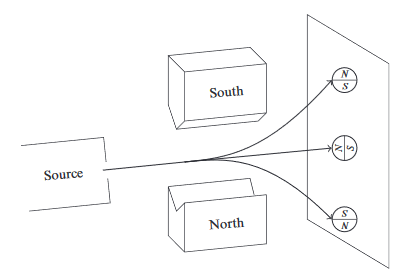
\includegraphics[width=0.6\textwidth]{images/1-Stern_Gerlach_Apparatus.png}
    \caption{Stern Gerlach apparatus \cite{bernhardt2019quantum}}
    \label{fig:stern-gerlach-apparatus}
\end{figure}

\subsection{Measurement}\label{ss:measurement}
The Stern Gerlach experiment is fundamental to quantum computing since it forms the basis of how qubits are measured. As the 1 and 0 in classical computing denotes a bit of information, spins in different directions represent a qubit. In Figure \ref{fig:stern-gerlach-apparatus} if we obtain a spin N in the vertical direction we will denote it with a 0 and if we obtain a spin S we can denote it with the binary digit 1 \cite{bernhardt2019quantum}. If we were to place one apparatus in the result of a first device we would obtain a string of N and S which when abstracted to represent 0 and 1 can be used to perform computations exactly in the same way as classical binary strings. Furthermore, if we were to rotate the second apparatus we would be obtaining a different measurement. In Figure \ref{fig:stern-gerlach-apparatus} the magnets are at a 90° degrees position but this angle can be changed, which in turn would affect the electromagnetic field thus changing the result of the measurement. Therefore, every time we measure a qubit by changing the angle of the measurement device we will obtain a different result \cite{bernhardt2019quantum}. \\

It is important to mention that following the theory of quantum mechanics the results of quantum measurements are completely random. This affirmation was largely discussed by physics who believed in the in the presence of unknown or hidden variables that affected the results of the results of quantum measurements \cite{einstein1971born} until it was demonstrated by Bell \cite{Bell1964} and Kochen and Specker \cite{kochen-specker1967} in 1964 and 1967 respectively that such variables couldn't exist. This introduces a fundamental difference with classical physics, which thinks of physical systems as deterministic, with a set of variables that if known at the time of measurement can predict the result of it. For example, if we toss a coin, knowing initial factors like the force of the toss, air resistance, weight of the coin, etc. we can predict and explain the result. Moreover, the problem of randomness is well known to computer scientists since classical computers are deterministic and cannot algorithmically generate truly random outputs. However, quantum systems are probabilistic, which means that their state can be completely random at the time of measurement \cite{bernhardt2019quantum}.
\subsection{Qubits}
Quantum computing and quantum mechanics concepts are formally described using vectors, therefore having an understanding of linear algebra is fundamental, specially when dealing with quantum gates and more complex concepts. The spin of a electron can be described using a linear combination of unit vectors in ${\mathbb{C}^n}$, but for the sake of simplicity and following the recommendations of Bernhardt \cite{bernhardt2019quantum} we will use units vectors in ${\mathbb{R}^2}$ in order to avoid the complications of complex numbers. \\

The formal representation of qubits in quantum computing also uses the notation created by English physicist Paul Dirac referred in the literature as Bra-Ket notation. The reason for the change is that physicists already use the concept of vectors to denote the relation between magnitudes and directions in the three-dimensional space whereas in the case of quantum theory (computing included) the vector describe the state of a quantum system.
We will start by defining how the Bra-Ket notation works and then deep dive into how qubits' states are represented. This notation uses angle brackets and vertical bars to abstract column or row vectors. For a column vector $\boldsymbol{a}$ and a given ket $\ket{a}$ we have.

\[\boldsymbol{a} = \begin{bmatrix}1 \\ 0 \end{bmatrix} = \ket{a} \]

Meanwhile for a given row vector $\boldsymbol{b}$ and a given bra ${\bra{b}}$ we would write it in the following way.

\[\boldsymbol{b} = \begin{bmatrix}1 & 0 \end{bmatrix} = \bra{b}\]

The next element that we have to introduce to understand qubits is probability. We already know that the two possible outcomes for our measurement are 1 and 0 generalized as $\ket{b_1}$ and $\ket{b_2}$, however since it can be any of these outcomes including both according to quantum mechanics fundamental principle of superposition \cite{dirac1947}, there is a probability amplitude attached to them that we will denote as $c_1$ and $c_2$. Finally a qubit state (noted as $\ket{\psi}$) can be given as the linear combination of its possible outcomes and the probabilities attached to both of them. \cite{bernhardt2019quantum}.
\begin{equation}\label{eq:1}
    \ket{\psi} = c_1\ket{b_1} + c_2\ket{b_2}
\end{equation}


Moreover, the probability that a qubit $\ket{\psi}$ is in state $\ket{b_1}$ is $c_1^2$ and the probability of it being in state $\ket{b_2}$ is $c_2^2$, where $c_1^2 + c_2^2 = 1$. \\

In classical computing every bit represents a $true$ or $false$ state, in probabilistic terms this would mean that when a bit is on state 1, the state $true$ has a 100\% probability of occurrence every time the bit is measured whereas the state $false$ has a 0\% chance of occurrence, the same logic can be applied in the opposite case. However, in the quantum theory a qubit can be in both states $true$ and $false$ with a certain degree of probability for each case, this superposition of states is explained in the next subsection. 

\subsection{Superposition}

As we have seen, probabilities affect the results of the measurement of a quantum system \cite{AllanAdams2013}.  Paul Dirac studied this phenomenon referring to it as the principle of superposition of states, he describes it as follows:

\begin{quote}
    The general principle of superposition of quantum mechanics applies to the states []... of any one dynamical system. It requires us to assume that between these states exist peculiar relationships such that whenever the system is definitely in one state we can consider it as being partly in each of two or more states. The original state must be regarded as the result of a kind of superposition of the two or more new states, in a way that cannot be conceived on classical ideas. Any state may be considered as the result of a superposition of two or more other states, and indeed in a infinite number of ways \cite{Dirac1967}...
\end{quote}
\begin{quote}
The non classical nature of the superposition process is brought out clearly if we consider the superposition of two states, A and B such that there exists an observation which, when made on the system in state A, is certain to lead to one particular result, a say, and when made on the system in state B is certain to lead to some different result, b say. What will be the result of the observation when made on the system in the superposed state? The answer is that the result will be sometimes a and sometimes b according to a probability law depending on the relative weights of A and B in the superposition state \cite{Dirac1967}
\end{quote}

The quantum system described above as a qubit $\ket{\psi} = c_1\ket{b_1} + c_2\ket{b_2} $ has only 2 states $\ket{b_1}$ and $\ket{b_2}$ which represent the binary states 1 and 0 respectively, but because we are dealing with elements governed by the principles of quantum theory one must assume that they can be in either of both or both. Mathematically we describe it by assigning a relative weight $c_1$ and $c_2$ respectively to each one of the states. \\

Superposition is a fundamental theoretical background of quantum computing and explains the vast potential of the technology by using the principle in two different ways. First, because a qubit can be in state 1 and 0, which is exactly the same function than a transistor has in our current computer architecture, any quantum computer would be able to behave as a classical computer \cite{bernhardt2019quantum}. Second, as demonstrated by Feynmann \cite{Feynman1982} Shor \cite{Shor1994} and Grover \cite{Grover1996}, since qubits can be in a superposition of states, they can perform calculations in parallel, allowing to solve problems with an exponential time-complexity much faster \cite{DeutschPenrose1985}.  

\subsection{Entanglement}\label{ss:entanglement}
In order for qubits to perform calculations simultaneously they also need to be related with each other. So far, we have operated using only one qubit for the sake of simplicity, but the reality is that for a quantum computer to be any useful it needs to have several of them. This is analogous to the idea that the more transistors a CPU has, the higher the complexity of operations it can perform by using these to build parallel processors. The way to perform this process in quantum computing is by entangling qubits.\\  

In simple terms, entanglement is defined as the relationship between two quantum systems $\ket{v}$ and $\ket{w}$ such that the measurement of $\ket{v}$ is highly correlated with the measurement of $\ket{w}$. Mathematically, this is represented by one particular result of the tensor product of $\ket{v}$ and $\ket{w}$, also noted as $\ket{v} \tens{} \ket{w}$. \\

Suppose that we have the qubits $\ket{v} = c_0\ket{a_0} + c_1\ket{a_1}$ and $\ket{w} = d_0\ket{b_0} + d_1\ket{b_1}$. If we compute their tensor product we would have:

\[\ket{v} \tens{} \ket{w} = (c_0\ket{a_0} + c_1\ket{a_1}) \tens{} (d_0\ket{b_0} + d_1\ket{b_1}) \]
\[\ket{v} \tens{} \ket{w} = c_0d_0\ket{a_0}\ket{b_0} + c_0d_1\ket{a_0}\ket{b_1} + c_1d_0\ket{a_1}\ket{b_0} + c1_d1 \ket{a_1}\ket{b_1} \]

We let $r = c_0d_0$, $s = c_0d_1$, $t = c_1d_0$ and $u = c_0d_0$.
\begin{equation}\label{eq:2}
   \ket{v} \tens{} \ket{w} = r\ket{a_0}\ket{b_0} + s\ket{a_0}\ket{b_1} + t\ket{a_1}\ket{b_0} + u\ket{a_1}\ket{b_1} 
\end{equation}

Where $r^2 + t^2 + s^2 + u^2 = 1$ as per the superposition principle. \\

From all of the possible combinations of $r, s, t$ and $u$ resulting in 1, when $ru \ne st$ we will refer to it as as being in an entangled state \cite{bernhardt2019quantum}. This inequality can be consistently achieved using quantum logical gates which will be introduced in the next chapter. \\

The results of equation \ref{eq:2} show that the combination of 2 qubits result in 4 different states, namely $\ket{a_0}\ket{b_0}, \ket{a_0}\ket{b_1}, \ket{a_1}\ket{b_0}$ and $\ket{a_1}\ket{b_1}$, with their respective probability of occurrence $r, s, t$ and $u$. Generalizing, entangled qubits have $2^n$ possible states each with a particular probability, where $n$ is the number of qubits of the machine. The power of quantum computing comes from favoring a certain probability within all of these possible states that are being computed simultaneously, this is also achieved by applying quantum logical gates on the qubits\cite{youtube:smith2018}.\\

Entanglement also allows us to perform a different kind of operation called quantum teleportation \cite{Ren2017} or superluminal communication \cite{bernhardt2019quantum}. Two qubits $\ket{v}$ and $\ket{w}$ that are entangled share a strong correlation among them such that if one measures $\ket{v}$ to be in state 0 ($\ket{0}$ in quantum computing notation), $\ket{w}$ will be in state 1 (noted $\ket{1}$), no matter how far apart the measurement takes place \cite{youtube:Morello2016}. Albert Einstein described this effect as a \textit{spooky action at a distance}, but it was proven by Bell's inequality \cite{Bell1964} that there was only a correlation without spookiness or any causality, it's just the probabilistic nature of quantum mechanics. In fact, several experiments have demonstrated quantum teleportation, one of them measuring entangled qubits' correlation separated by a distance of 1400km from ground to a satellite in the space with a fidelity of 80\% \cite{Ren2017}. This kind of information teleportation would enable instant and secure communications between distant places, powering quantum communications methods like Quantum Key Distribution
\footnote{Figure \ref{fig:qkd} shows how Quantum Key Distribution allows two communicating parties to securely share encrypted keys by using entangled photons. The process is described by Diamanti \cite{Diamanti2017} as follows: \textit{To achieve this, the authors produced a pair of photons (X and Y) that were entangled — a condition whereby measuring the state of one particle determines the state of the other — and sent photon X to the satellite (orange arrow). They then performed a joint measurement of photon Y and a third photon (Z), whose polarization state was to be teleported. Finally, they used the outcome of this measurement to determine whether the polarization of photon X had been transformed into the polarization of photon Z (green arrow)".}}
which in turn could lead to the development of a Quantum Internet.
\begin{figure}[ht]
    \caption{Long Distance Quantum Communication \cite{Diamanti2017}.}
    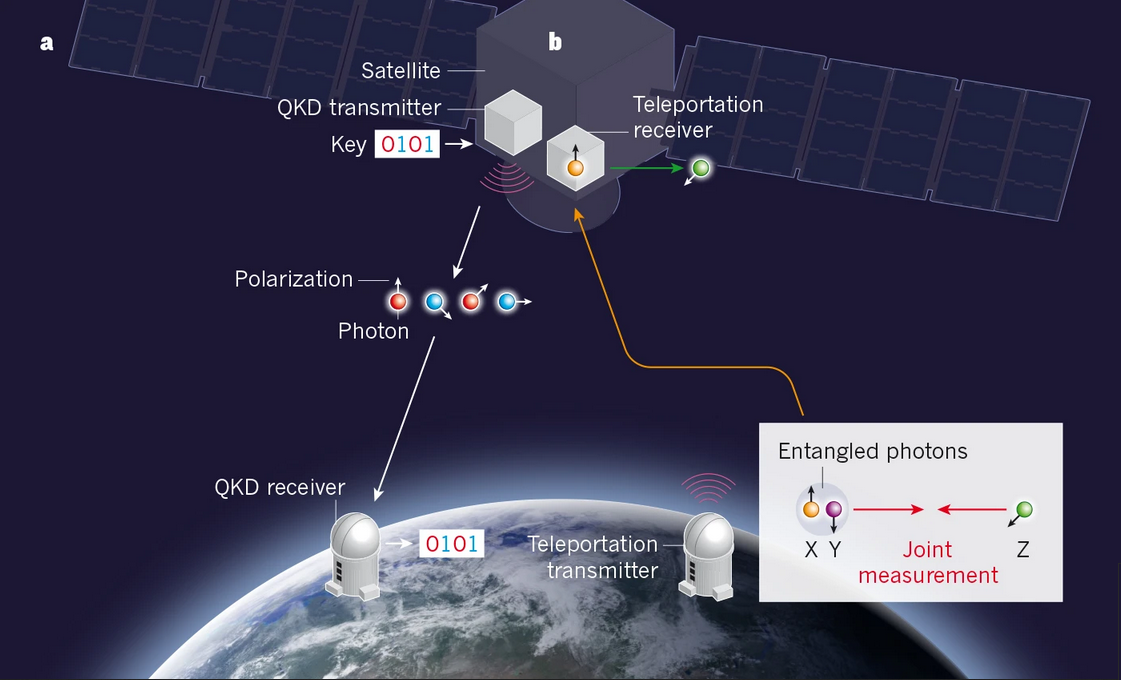
\includegraphics[width=0.8\textwidth]{images/2-QKD_diagram.png}
    \label{fig:qkd}
\end{figure}

\section{Quantum Computing}

The main objective of this chapter is to introduce the reader into how quantum computers operate from a logical standpoint by establishing similarities and comparisons between classical and quantum computing. The composition and physical workings of quantum computing hardware are out of the scope of this publication.\\

Classical computing relies on boolean algebra to build circuits which are the basic building blocks of processors. As discussed previously, boolean algebra is suitable for these calculations since it's adapted to the way that a bit is represented: by the presence or absence of electricity within a circuit, this binary state maps to boolean states $True$ and $False$ respectively. Boolean algebra define operations whose inputs and outputs are assorted from \textit{truth tables}, a representation of the mathematical relation between a pair of inputs that produce a particular output. All these operations can be performed with electrical switches whose combination produces logical gates, completing the basic idea behind circuits \cite{bernhardt2019quantum}. \\

The most basic logical gates are the $NOT$, $AND$ and $OR$ gate, whose truth table is represented on figure \label{table:truthtablevarious}. But in order to make our computations more efficient, we have to consider two properties of boolean algebra applied to gates, functional completeness and reversibility \cite{bernhardt2019quantum}. A gate is functional complete or universal when it can implement any boolean function by itself, like the $NAND$ gate, which is built by combining an $AND$ gate whose output is inverted by a $NOT$ gate \cite{Bourdillon1985}, using this gate we can build any computer since we can implement any boolean function efficiently. The reversibility concept is a property of those gates that do not lose any information, they take $n$ number of inputs and return $n$ number of outputs, and by knowing an output one can deduce their inputs, this concept is opposed to the result of an $AND$ gate which takes two inputs and produces one output. The $CNOT$ gate is an example of a reversible gate. These two properties, while relevant for the efficiency of traditional computation will be equally important in quantum computation since the theory behind quantum logical gates is founded on them.\\

%Figures of AND, NOT, OR gates and NAND and CNOT    
\begin{figure}[H]
    \centering
    \begin{tabular}{|c|c|c|c|c|c|c|} 
    \hline
    $a$ & $b$ & $\lnot{a}$ &$a\wedge{b}$ & $a\lor{b}$ & $a|b$ & $a$ $CNOT$ $b$ \\
    \hline
    T & T & F & T & T & F & [F, F] \\
    T & F & F & F & T & T & [T, T] \\
    F & T & T & F & T & T & [F, T] \\
    F & F & T & F & F & T & [T, F] \\
    \hline
    \end{tabular}
    \caption{Truth tables for NOT, AND, OR, NAND and CNOT operators}
    \label{table:truthtablesvarious}
\end{figure}


\subsection{Quantum Gates}\label{section_quantum_gates}

As explained in the chapter's introduction, circuits rely on the presence or absence of electricity to perform logical operations. Electricity is an abstraction of a quantum process \cite{Longair2013}, therefore we cannot rely on it when dealing with quantum elements. However, the same binary result can be achieved by the spin of an electron or the polarisation of a photon. \\

Since we can achieve the same binary states by abstracting these quantum processes as described in sections \ref{ss:quantum_spin} and \ref{ss:measurement}, we can also implement the principles of boolean algebra that allow to perform computations. Using quantum logical gates can be thought of as rotating the measuring device in the Stern-Gerlach experiment after each measurement, mathematically this is represented by multiplying the qubits by an orthogonal matrix \cite{bernhardt2019quantum}. \\

It is important to mention that there can be infinitely many quantum gates, because the number of degrees that we can rotate the apparatus to measure qubits is also infinite. This is a fundamental difference with classical computing where there is only a limited set of logical operations that can be performed on a given input. However, there are some gates that are worth mentioning since they have special outputs, these are the Hadamard gate, the CNOT gate and the Pauli Transformations, we will focus in the first two.

\subsubsection{Hadamard Gate}

The Hadamard gate is used to put qubits in a superposition state $\ket{\psi} = c_1\ket{b_1} + c_2\ket{b_2}$ where $c_1^2 + c_2^2 = 1$. It is defined by the letter \textbf{H} and represented as a $2*2$ orthogonal matrix.


\begin{equation}
 \boldsymbol{H} = \begin{bmatrix}\frac{1}{\sqrt{2}} &  \frac{1}{\sqrt{2}} \\ \frac{1}{\sqrt{2}} & -\frac{1}{\sqrt{2}} \end{bmatrix}
\label{gate:hadamard}   
\end{equation}

Suppose we have a random qubit state defined by $\ket{0}$, after applying the Hadamard gate we get.

\[H(\ket{0})  = \begin{bmatrix}\frac{1}{\sqrt{2}} &  \frac{1}{\sqrt{2}} \\ \frac{1}{\sqrt{2}} & -\frac{1}{\sqrt{2}} \end{bmatrix} \tens{} \ket{0}\]
\[H(\ket{0})  = \begin{bmatrix}\frac{1}{\sqrt{2}} &  \frac{1}{\sqrt{2}} \\ \frac{1}{\sqrt{2}} & -\frac{1}{\sqrt{2}} \end{bmatrix} \tens{} \begin{bmatrix} 1 \\ 0 \end{bmatrix}\]
\[H(\ket{0})  = \begin{bmatrix}\frac{1}{\sqrt{2}}  \\ \frac{1}{\sqrt{2}} \end{bmatrix} = \frac{1}{\sqrt{2}}\ket{0} + \frac{1}{\sqrt{2}}\ket{1}\]

Notice how the qubit enters a superposition state where there is a probability of $\frac{1}{2}$ that after measurement this will be in state $\ket{0}$ and a probability of $\frac{1}{2}$ that will be measured to $\ket{1}$. The same logic can be applied to a qubit on state $\ket{1}$.

\[H(\ket{1})  = \begin{bmatrix}\frac{1}{\sqrt{2}} &  \frac{1}{\sqrt{2}} \\ \frac{1}{\sqrt{2}} & -\frac{1}{\sqrt{2}} \end{bmatrix} \tens{} \ket{1}\]
\[H(\ket{0})  = \begin{bmatrix}\frac{1}{\sqrt{2}} &  \frac{1}{\sqrt{2}} \\ \frac{1}{\sqrt{2}} & -\frac{1}{\sqrt{2}} \end{bmatrix} \tens{} \begin{bmatrix} 0 \\ 1 \end{bmatrix}\]
\[H(\ket{0})  = \begin{bmatrix}\frac{1}{\sqrt{2}}  \\ -\frac{1}{\sqrt{2}} \end{bmatrix} = \frac{1}{\sqrt{2}}\ket{0} - \frac{1}{\sqrt{2}}\ket{1}\]

In this case even though the state $\ket{1}$ is negative that doesn't pose any problem when verifying the superposition property $c_1^2+c_2^2=1$.
\[(\frac{1}{\sqrt{2})})^2 + (-\frac{1}{\sqrt{2})})^2 = 1\]



\subsubsection{CNOT gate}

One of the most used gates in quantum computing is the $CNOT$ gate because it has the property of entangling qubits, $CNOT$'s gate matrix representation is given by.

\begin{equation}
 \boldsymbol{CNOT} = 
 \begin{bmatrix}
 1 &  0 & 0 & 0 \\ 
 0 &  1 & 0 & 0 \\
 0 &  0 & 0 & 1 \\
 0 &  0 & 1 & 0 
 \end{bmatrix}
\label{gate:cnot}   
\end{equation}

The operation performed by the CNOT gate allows two input qubits outputting a control qubit plus the tensor product of both.  This operation entangles qubits by creating a relation between both qubits as described in section \ref{ss:entanglement}. A truth table built with these results is given below.

\begin{table}[H]
\centering
\begin{tabular}{|c|c|c|c|} 
 \hline
\multicolumn{2}{|c|}{Input} & \multicolumn{2}{|c|}{Output} \\
\hline
$x$ & $y$ & $x$ & $x\tens{}y$ \\
\hline
$\ket{0}$ & $\ket{0}$ & $\ket{0}$ & $\ket{0}$ \\
\hline
$\ket{0}$ & $\ket{1}$ & $\ket{0}$ & $\ket{1}$ \\
\hline
$\ket{1}$ & $\ket{0}$ & $\ket{1}$ & $\ket{1}$ \\
\hline
$\ket{1}$ & $\ket{1}$ & $\ket{1}$ & $\ket{0}$ \\
\hline
\end{tabular}
\caption{CNOT Gate truth table \cite{bernhardt2019quantum}}
\label{table:cnot}
\end{table}

Using a more compact notation to describe the tensor product the table can be also represented as follows.

\begin{table}[H]
\centering
\begin{tabular}{|c|c|} 
 \hline
Input & Output \\
\hline
$\ket{00}$ & $\ket{00}$ \\
\hline
$\ket{01}$ & $\ket{01}$ \\
\hline
$\ket{10}$ & $\ket{11}$  \\
\hline
$\ket{11}$ & $\ket{10}$ \\
\hline
\end{tabular}
\caption{CNOT Gate truth table using compact notation \cite{bernhardt2019quantum}}
\label{table:cnot-compact}
\end{table}

A fundamental application of quantum logical gates is the  creation of a Bell state, where the output of a Hadamard gate is put into a $CNOT$ gate, consistently achieving an entangled spin state and forming the basis of several quantum applications. Among these we can mention superdense coding, quantum teleportation (as described in section \ref{ss:entanglement}) and cryptographic quantum algortihms. Figure \ref{fig:bellstate} describes a Bell state also known as Bell circuit. 

\begin{figure}[H]
    \centering
    \begin{quantikz}
    \lstick{$\ket{0}$} & \gate{H}& \ctrl{1} & \qw \rstick[wires=2]{$\frac{1}{\sqrt{2}}\ket{00} + \frac{1}{\sqrt{2}}\ket{11}$} \\
    \lstick{$\ket{0}$} & \qw &\targ{} & \qw 
    \end{quantikz}
    \caption{Bell State for inputs $\ket{0}, \ket{0}$}
    \label{fig:bellstate}
\end{figure}

We will mathematically explain the result of figure \ref{fig:bellstate} and the reader will perform the same operations to verify the rest of possible combinations between 2 qubits. First we apply a Hadamard gate to a qubit $\ket{0}$. \\

\[H(\ket{0})  = \frac{1}{\sqrt{2}}\ket{0} + \frac{1}{\sqrt{2}}\ket{1}\]
We then multiply the result by the second input of the $CNOT$ gate. 
\[
    (\frac{1}{\sqrt{2}}\ket{0} + \frac{1}{\sqrt{2}}\ket{1}) \tens{} \ket{0} =
    \frac{1}{\sqrt{2}}\ket{0}\ket{0} + \frac{1}{\sqrt{2}}\ket{1}\ket{0}
\]

Applying the CNOT gate as per its truth table evaluates to $\ket{0}\ket{0} \rightarrow \ket{0}\ket{0} $ and $\ket{1}\ket{0} \rightarrow \ket{1}\ket{1}$. After applying the compact notation we finally we have our entangled qubits.

\begin{equation}
    (\frac{1}{\sqrt{2}}\ket{0} + \frac{1}{\sqrt{2}}\ket{1}) \tens{} \ket{0} =
    \frac{1}{\sqrt{2}}\ket{00} + \frac{1}{\sqrt{2}}\ket{11}
\end{equation}

Ultimately, as it is the case with classical computing behind the layers of abstraction created by the processor and the operating system, developing quantum algorithms involves combining different logical gates to achieve a particular computation. 

\subsection{Quantum Algorithms}\label{ss:quantumalgorithms}

The core value proposition of quantum computers consist in an increased speed up in calculations compared to traditional ones. This is achieved due to qubits being in a superposition of all possible states which allows algorithms to run on every possible output simultaneously \cite{bernhardt2019quantum}. In order to find the right result of the algorithm, the programmer relies on the probabilities of these superposed states, introducing a fundamental difference between both computational models.\\

According to the time complexity theory \cite{goodrich2001algorithm}, the time required to measure the speed of an algorithm is measured in terms of the length of its input, represented by a letter $n$ \cite{goodrich2001algorithm}. Subsequently, solvable algorithms can be run in either polynomial (e.g. $n+3$) or exponential time (e.g. $2^n$), a set of the latter attempt to solve intractable problems, or algorithms that attempt to resolve problems that would take so long to complete computation for large values of $n$ that their implementation is impractical. Within these we encounter problems that can be solved in non-deterministic polynomial time (NP), these are problems whose time complexity is exponential but could be solved in polynomial time by a non deterministic machine. Due to the non deterministic nature of quantum mechanics these problems are in theory solvable by quantum computers \cite{bernhardt2019quantum}.\\

David Deutsch demonstrated in 1985 that a quantum algorithm could solve problems faster than a classical one \cite{DeutschPenrose1985}, confirming that quantum computers could solve NP problems. This algorithm is today known as Deutsch algorithm and involves evaluating functions of one variable and deciding if such function is constant or balanced.
In order to understand Deutsch algorithm we have to define four boolean functions who outputs are define in the following table.

\begin{table}[H]
    \centering
    \begin{tabular}{|c|c|c|c|c|}
        \hline
         input & $f_0$ & $f_1$ & $f_2$ & $f_3$  \\
         \hline
          0    &   0   & 0    &   1    & 1        \\
          \hline
          1    &   0  &   1    &   0    & 1  \\
          \hline
    \end{tabular}
    \caption{Deutsch Algorithm's functions}
    \label{tab:deutsch.functions}
\end{table}

The functions $f_0$ and $f_3$ are constant, which means that the output is the same for both functions regardless of the input. On the other hand, $f_1$ and $f_2$ are balanced since it evaluates its inputs to 0 and 1 with a probability of $1/2$ respectively. \\

The classical approach in order to determine whether the function is constant or balanced. Involves evaluating the function two times, one per each input. If the function evaluates two times to 0 or 1, we will know it is constant and if it evaluates to 1 and then to 0 or viceversa, we will know that it is balanced. \\

The quantum solution of the algorithm only needs one evaluation to produce the correct output \cite{DeutschPenrose1985}. It achieves this by leveraging the superposition states of two qubits which go through a quantum gate known as Quantum Oracle called $F_i$. A Quantum Oracle is a black-box function that will be interrogated in terms of the results that we want to achieve. In the case of Deutsch's algorithm the oracle will be asked whether our function is balanced or constant.

\begin{figure}[H]
    \centering
    \begin{quantikz}
    \lstick{$\ket{0}$} & \gate{H} &    \gate[wires=2]{\text{$F_i$}} \ctrl{1} & \gate{H} & \meter{measurement} \arrow{r} & \rstick{\text{$\ket{1} \lor{\ket{0}}$}}  \\
    \lstick{$\ket{1}$} & \gate{H} & \ctrl{} & \qw & \qw & \trash{\text{trash}} \\ 
    \end{quantikz}
    \caption{Deutsch Algorithm's quantum circuit}
    \label{fig:deutschalgorithmquantumcircuit}
\end{figure}

Figure \ref{fig:deutschalgorithmquantumcircuit} shows the quantum circuit for Deutsch's algorithm in which, as a first step, both qubits go through Hadamard gates, superposing their states as follows:
\[ \boldsymbol{H}(\ket{0}) \frac{1}{\sqrt{2}}(\ket{0} + \ket{1}) \] and
\[ \boldsymbol{H}(\ket{1}) \frac{1}{\sqrt{2}}(\ket{0} - \ket{1}) \]

Since the system involves two qubits we have to calculate the tensor product of both terms in order to be able to work with them \cite{bernhardt2019quantum}.

\[ \boldsymbol{H}(\ket{0}) \tens{} \boldsymbol{H}(\ket{1}) = \frac{1}{2}(\ket{00} - \ket{01} + \ket{10} - \ket{11}) \]

Subsequently qubits go through the $F_i$ gate \footnote{Also known as F-CNOT gate in the literature.}, which consists of a tensor product of the qubits and the functions containing the second qubit as input. Note that  $i$ represents one of the four possibilities for evaluating $f(x)$ as referred in table \ref{tab:deutsch.functions}.

\begin{equation}
    \boldsymbol{F_i}(\frac{1}{2}(\ket{00} - \ket{01} + \ket{10} - \ket{11})) =  \frac{1}{2}(\ket{0}\tens{}\ket{f_i(0)}-\ket{0}\tens{}\ket{f_i(0)\oplus{1}}+\ket{1}\tens{}\ket{f_i(1)}-\ket{1}\tens{}\ket{f_i(1)\oplus{1}})
\end{equation}

After some mathematical transformations that can be found in Bernhadt's Quantum Computing for Everyone \cite{bernhardt2019quantum}, we end up with the following expression for the top qubit.

\begin{equation}
    \frac{1}{\sqrt{2}}((-1)^{f_i(0)}\ket{0}+(-1)^{-f_i(1)}\ket{1})
\end{equation}

At this point, we can start to evaluate $f_i(0)$ by assigning $f$ all of the possible outputs\footnote{This is analogous to say that we we are interrogating the Oracle}. For $f_1(0)$ for example, the qubit will be in the state $\frac{1}{\sqrt{2}}(\ket{0} + \ket{1})$. The rest of the results can be found in table \ref{tab:deutsch.quantum_intermediate}.

\begin{table}[H]
    \centering
    \begin{tabular}{|c|c|c|c|c|}
        \hline
         input & $f_0$ & $f_1$ & $f_2$ & $f_3$  \\
         \hline
          0    &   $\frac{1}{\sqrt{2}}(\ket{0} + \ket{1})$   & $\frac{1}{\sqrt{2}}(\ket{0} - \ket{1})$    &   $-\frac{1}{\sqrt{2}}(\ket{0} - \ket{1})$    &  $-\frac{1}{\sqrt{2}}(\ket{0} + \ket{1})$        \\
          \hline
          1    &   $\frac{1}{\sqrt{2}}(\ket{0} + \ket{1})$   & $\frac{1}{\sqrt{2}}(\ket{0} - \ket{1})$    &   $-\frac{1}{\sqrt{2}}(\ket{0} - \ket{1})$    &  $-\frac{1}{\sqrt{2}}(\ket{0} + \ket{1})$      \\
          \hline
    \end{tabular}
    \caption{Deutsch Algorithm. Qubit evaluation after passing through the $F$ gate.}
    \label{tab:deutsch.quantum_intermediate}
\end{table}

Following the $F_i$ gate we ignore the bottom qubit and pass the top qubit through the Hadamard gate, which, thanks to the reversibility property (As discussed in section \ref{section_quantum_gates}) will revert the superposition and set a single qubit to the value $\ket{1}$ or $\ket{0}$. For each of the functions the Hadamard gate returns \\

\begin{table}[H]
    \centering
    \begin{tabular}{|c|c|}
        \hline
         Function & Hadamard Result  \\
          \hline
         $f_0$ & $\ket{0}$ \\
          \hline
        $f_1$ & $\ket{1}$ \\
         \hline
        $f_2$ & $-\ket{1}$ \\
         \hline
        $f_3$ & $-\ket{0}$ \\
         \hline
    \end{tabular}
    \caption{Deutsch Algorithm. Qubit state after passing through the final Hadamard gate.}
    \label{tab:deutsch.quantum_hadamard2}
\end{table}

The final step of the algorithm is the measurement (See figure \ref{fig:deutschalgorithmquantumcircuit}), and we can notice that both functions $f_0$ and $f_3$ will measure to 0 while $f_1$ and $f_2$ will measure to 1 for any of its inputs. If we get 0 we know that the function was constant and if we get 1 it's certain that the function was balanced \cite{bernhardt2019quantum}. In conclusion, we only need to evaluate the function once in order to give the correct result instead of the two evaluations that we took with a deterministic algorithm. \\

We have seen how a quantum algorithm is implemented using quantum gates and qubits, even though Deutsch's algorithm doesn't give any particularly useful result it is a demonstration of the power of quantum computations and particularly a display of how superposition can offer results faster than deterministic polynomial algorithms. Moreover, Deutsch and Richard Josza generalized this algorithm for n-bits inputs in the Deutsch-Josza Algorithm, but it still has no practical use. More useful and advanced algorithms have been developed by Shor \cite{Shor1994} in the field of cryptography and Groover \cite{Grover1996} in database search. Unfortunately, due to their mathematical complexity, they are out of the scope of this work. Next chapter will show how the mathematical model explained in this section can be implemented in a real quantum simulator using a software development kit called Qiskit \cite{qiskit}. 

\section{Quantum Algorithm implementation on the IBM Q Cloud Experience}

Implementing an algorithm on a quantum computer require us to understand how this is built. Figure \ref{fig:qc-layers} displays a layer cake were the elements needed on a quantum architecture are categorised into 5 layers that cover the process of running an algorithm within quantum hardware. Even though that the approach to build quantum computers is slightly different depending on the manufacturer, they all share similarities that can be found in this approach built by Qutech Research Institute in the Netherlands \cite{versluis2020}. 

\begin{figure}[H]
    \centering
    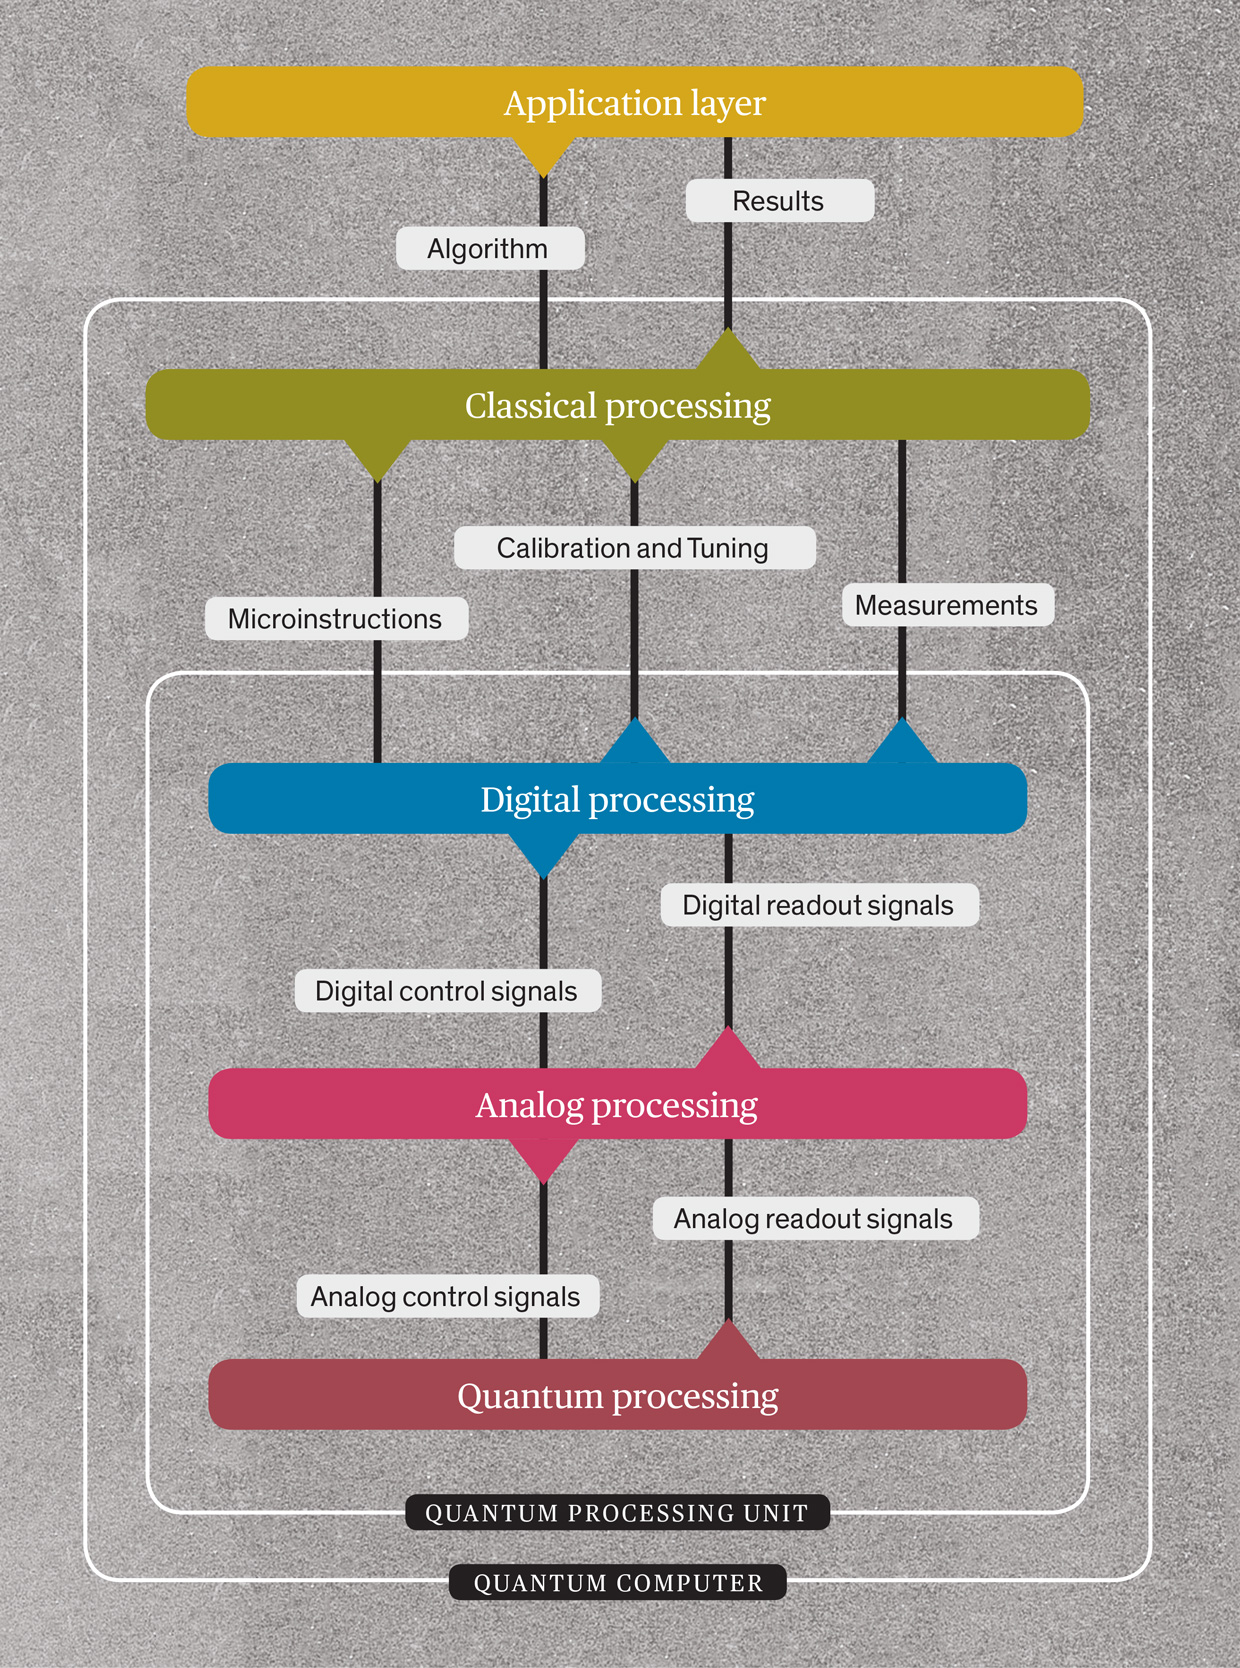
\includegraphics[width=0.4\textwidth]{./images/3-quantum_computing_layers}
    \caption{Quantum Computer Layer Cake \cite{versluis2020}}
    \label{fig:qc-layers}
\end{figure}

At the top of the diagram we can find the application layer which involves all the software required for the machine to work, like the operating system, programming environment, user interfaces, etc. The goal of this layer is to produce an algorithm, that can be classical or quantum or a mixture of both. The next layer is known as Classical Processing and has two main functions. First, the quantum algorithm is compiled into microinstructions for the Quantum Processing Unit (QPU) and second, it processes the results of the the qubits' measurement. On this layer we can see the interaction between classical and quantum computation, which is needed in order to leverage our current computing model and benefiting from the augmentation given by quantum computations.\\

The next three layers are contained by the QPU and are so tightly coupled that can look different depending on the hardware. Within the Digital Processing layer instructions are translated to electromagnetic pulses which represent the quantum logical gates that are applied in order to manipulate qubits, this layer also translates back the results of the measurement to the classical processing layer in order to be able to continue the calculations using the classical computing approach. The layer in charge of actually producing, emitting and receiving these electromagnetic signals is the Analog Processing layer, they are applied directly to the qubits contained by the Quantum Processing layer. The results of the qubit's interaction within the Quantum processing layer are read back by the Analog Processing layer in order to be sent all the way back to the Application layer.

\subsection{IBM Q System One}

IBM is one of the various quantum computer producers that are competing to offer the power of quantum computations to an array of commercial industries such as chemical, finance, medical, biological among others. In January 2019, they presented the first integrated quantum computing system for commercial use, called the IBM Q System One \cite{IBMPress012019} which aims to reduce the complexity of quantum computing by offering an all-in-one solution for using the power of quantum. The system is composed by quantum hardware containing 20 physical qubits \cite{HCP2019}, cryogenic engineering for stabilizing the qubits, quantum firmware to control the QPU and a set of classical computation tools that allow developers to access the quantum hardware through the cloud using a software development kit (SDK) called Qiskit, which has all the features needed to implement quantum algorithms. The computer together with quantum simulators and programming interfaces needed are available to the general public via the IBM Quantum Experience, that allows developers from all over the world to experiment with quantum algorithms for free \cite{ibm-q-e}.

\subsection{Qiskit}

Qikit was developed by IBM under an open source licence in order to provide programmers access to quantum hardware. It implements the set of Quantum Gates and circuits most frequently used for building quantum algorithms. It is written in Python and has an extensive documentation with several use cases implemented using Jupyter Notebooks on the IBM Quantum Experience. Qiskit is available through different package managers like Conda and Pipy as well as a ready to use version in the IBM Quantum Experience. \\

Among the possibilities that Qiskit offers, it allows to interact directly with quantum hardware using a set of standardized machine instructions known as OpenQSAM \cite{QSAM} aimed at developing new quantum algorithms using well defined universal gates and circuits. At the same time it offers a framework called Qiskit Aqua which implements the quantum programming model through a library of algorithms that can be used in domain-specific applications \cite{QiskitAqua}. 

\subsection{Deutsch Algorithm Implementation in the IBM Quantum Experience}
%http://akyrillidis.github.io/notes/quant_post_8
%
The IBM Quantum Experience \cite{ibm-q-e} allows to run quantum algorithms via cloud using Jupyter notebooks and Qiskit's SDK, it also provides a graphical interface to compose circuits. In this section we will implement the Deutsch Algorithm described mathematically in chapter \ref{ss:quantumalgorithms} which will allow us to understand how to program a quantum computer. The IBM Quantum Experience would form part of the application layer showed in figure \ref{fig:qc-layers}, since it interfaces between the programmer and the quantum computer. In this case, we will make use of a quantum simulator that enables to run job's using a few qubits simulated by a classical computer. This approach works until the amount of qubits is sufficiently large to make the classical hardware unable to calculate the states probabilities, once this barrier is reached, the literature describes it as having achieved Quantum Supremacy \cite{Arute2019}.\\

In this article we will focus in the Jupyter notebook implementation since it allows us to understand better the step by step process for executing the algorithm, the reader can refer to figure \ref{fig:deutschalgorithmquantumcircuit} in order to have a graphical representation and compare with the Python code. The complete source implementation of this algorithm can be found Murat Koptur's Github repository \cite{kopturgithub}.

After creating an IBM account and opening a new Jupyter Notebook, we start by importing the libraries needed to reach the quantum computer and loading our IBM account to identify ourselves within the system.

\begin{lstlisting}[language=python]
from qiskit import IBMQ, BasicAer
from qiskit.providers.ibmq import least_busy
from qiskit import QuantumCircuit, ClassicalRegister, QuantumRegister, execute
from qiskit.tools.monitor import job_monitor
from qiskit.compiler import transpile, assemble
from qiskit.tools.jupyter import *
from qiskit.visualization import *
provider = IBMQ.load_account()
\end{lstlisting}

We will proceed to initialize the qubits and bits needed for this computation. In this case, we need 2 qubits and 2 classical bits in order to store the results. We also need to create a circuit with these two elements, analog to the circuit in figure \ref{fig:deutschalgorithmquantumcircuit}.

\begin{lstlisting}[language=python]
qr = QuantumRegister(2)  
cr = ClassicalRegister(2) 
circuit = QuantumCircuit(qr, cr)
\end{lstlisting}

In order to run the algorithm properly, the bottom bit in figure \ref{fig:deutschalgorithmquantumcircuit} needs to be initialised to $\ket{1}$. For this operation we need to apply an X-Gate, which forms part of the Pauli transformations and basically sets the qubit to state $\ket{1}$. After this step, Qiskit requires us to impose barriers in order to isolate the execution of each step.

\begin{lstlisting}[language=python]
circuit.x(qr[1]) 

circuit.barrier()
\end{lstlisting}
We apply a Hadamard gate to both qubits in order to reach a superposition state.
\begin{lstlisting}[language=python]
circuit.h(qr[0])
circuit.h(qr[1])

circuit.barrier()
\end{lstlisting}
Now we will implement the Oracle function. Since we want to know whether the function is constant or balanced, we can ask the Oracle whether our function is balanced by applying a CNOT Gate. 
\begin{lstlisting}
circuit.cx(qr[0], qr[1])

circuit.barrier()
\end{lstlisting}

As the next step, a hadamard gate is applied to the top qubit in order to revert the superposition of states.
\begin{lstlisting}
circuit.h(qr[0])

circuit.barrier()
\end{lstlisting}
Finally we measure the top qubit in order to check the results of the algorithm.

\begin{lstlisting}
circuit.measure(qr[0], cr[0])
\end{lstlisting}

In order to output our results we have to set up the machine to use the simulator for executing the quantum algorithm and load the measurement into the classical processing layer (See figure \ref{fig:qc-layers}). This would give us an answer in terms of classical bits that we can interpret accordingly.

\begin{lstlisting}[language=python]
backend = BasicAer.get_backend('qasm_simulator')
shots = 1024 #Specifies the number of times the circuit be executed 
results = execute(circuit, backend=backend, shots=shots).result()
answer = results.get_counts()
print(answer) #{'01': 1024}
\end{lstlisting}
The answer obtained indicates that the qubit measured is on state $\ket{1}$ during a total of 1024 executions. If we refer to table \ref{tab:deutsch.quantum_hadamard2}, we will find that for a balanced function the Hadamard result returns a string '01' or $\ket{1}$. This confirms the quantum result of Deutsch algorithm where a function has to be evaluated only once in order to determine if it's balanced or constant. If we would like to verify the algorithm for the simplest case of constant functions, we would omit the CNOT gate, which would give us the following.

\begin{lstlisting}[language = python]
qr = QuantumRegister(2)  
cr = ClassicalRegister(2) 
circuit = QuantumCircuit(qr, cr)

circuit.x(qr[1]) 

circuit.barrier()

circuit.h(qr[0])
circuit.h(qr[1])

circuit.barrier()

circuit.barrier()
circuit.h(qr[0])
circuit.measure(qr[0], cr[0])

backend = BasicAer.get_backend('qasm_simulator')
shots = 1024 #Specifies the number of times the circuit be executed 
results = execute(circuit, backend=backend, shots=shots).result()
answer = results.get_counts()
print(answer) #{'00': 1024}
\end{lstlisting}

As we can notice, the oracle oracle function returns $\ket{0}$ for a constant function with input 0. From this result we can conclude that the oracle function determines the results of the algorithm\footnote{This is also the case in most of quantum algorithms.} and that implementing a different oracle function for each one of the functions will yield a result, according to table \ref{tab:deutsch.quantum_hadamard2}. The reader can refer to the following stack-exchange question for the implementation of the remaining oracle functions \cite{veseli2020}.


\section{Conclusion}
This report describes the fundamental concepts involved in programming a quantum computer. Since quantum programming introduces a fundamental change of paradigm on how to perform computations due to it's probabilistic nature, the programmer has to know how to work with these probabilities and modify them according to the desired results. It is fundamental for programmers to understand the quantum physics concepts applied to computations like superposition, entanglement or measurement and secondly the effect that quantum gates and circuits have on qubits, because they are a constant in every quantum algorithm. Furthermore, programmers need to understand the mathematics behind existing algorithms in order to use them effectively for their purposes and apply them to their own applications, but it is probable that this need will be reduced  with the time as more tools and abstractions are developed in order to make quantum computers easier to use. One example of the latter is the IBM Quantum Experience, which allows us to implement existing algorithms and analyse their results but unfortunately, these still cannot be used in productions applications due to the lack of qubits needed to produce useful outputs that arise from millions of possible simultaneous states. Even though we are at an early stage in the technology, the fact that tools like this one are already made available to programmers all over the world represents a significant potential for the development of new applications and algorithms.\\
Further work into the topic would require us to present and analyse in depth certain concepts (e.g. no-cloning theorem or superdense coding) algorithms (Shor and Groover algorithms) that even though they are fundamental knowledge steps of quantum programming were omitted in this article due to their length and complexity. The reason for this being that the author wanted to remove all the non essential information to understand how quantum programming works, with the objective of making the topic more accessible and produce an easy to follow guide in order to get started with quantum programming. Finally, another fundamental topic that was not mentioned on this article due to the reason mentioned above but that has to be researched further is qubit error correction and its implications, which is one the most fundamental challenges that quantum programming has at the moment \cite{bernhardt2019quantum}.

\markboth{}{}

\newpage

\bibliographystyle{plain} % We choose the "plain" reference style
\bibliography{bibli} % Entries are in the "bibi.bib" file




\newpage
\thispagestyle{empty}
\markboth{}{}
  \normalsize
\begin{center}
\huge{\textbf{ Declaration of Independence}}\\[40mm]
\end{center}
\large
I affirm that the above work has been produced by myself without any unauthorized assistance and without the use of any other means than those indicated, and that I have marked as such all passages that have been taken literally or meaningfully from published or unpublished writings.\\[50mm]
Bienne, the \today

\newpage



\end{document}